\documentclass[newPxFont,noprogressbar,table]{beamer}
%\documentclass[newPxFont,sthlmFooter]{beamer}

%\documentclass[border=3mm,tikz,preview]{standalone}
%\usetikzlibrary{calc,backgrounds,positioning,fit}


\usetheme{sthlm}
%\usecolortheme{sthlmv42}

\setbeamertemplate{footline}[frame number]

%-=-=-=-=-=-=-=-=-=-=-=-=-=-=-=-=-=-=-=-=-=-=-=-=
%        LOADING PACKAGES
%-=-=-=-=-=-=-=-=-=-=-=-=-=-=-=-=-=-=-=-=-=-=-=-=
\usepackage[utf8]{inputenc}


% ADDED PACKAGES
%//////////////////////////////////////////////////////

\usepackage{helvet}
\renewcommand{\familydefault}{\sfdefault}

\usepackage[utf8]{inputenc}
%\usepackage[absolute,overlay]{textpos}
% Booktabs
\usepackage{booktabs}
\usepackage{multirow}
\usepackage{subfig}
% Algorithm package
\usepackage{algpseudocode} % Typesetting using the algorithmicx package
\renewcommand{\algorithmiccomment}[1]{\bgroup\hfill//~#1\egroup} % Algorithm comment

\usepackage{graphicx}
\usepackage{epstopdf}

\epstopdfDeclareGraphicsRule{.gif}{png}{.png}{convert gif:#1 png:\OutputFile}
\AppendGraphicsExtensions{.gif}

\setlength{\tabcolsep}{5pt}

% For floating point columns
\usepackage{etoolbox} 
\usepackage[tight-spacing=true]{siunitx}
\robustify\bfseries
% For bold cells using siunitx
\newcommand{\be}[2]{%
	%	\multicolumn{1}{S[table-format=#1,
	\multicolumn{1}{>{\columncolor[HTML]{FFCE93}}S[table-format=#1,
		mode=text,
		text-rm=\fontseries{b}\selectfont
		]}{#2}}

% For bold cells using siunitx
\newcommand{\beUpperBound}[2]{%
	%	\multicolumn{1}{S[table-format=#1,
	\multicolumn{1}{>{\columncolor[HTML]{32CD32}}S[table-format=#1,
		mode=text,
		text-rm=\fontseries{b}\selectfont
		]}{#2}}


% Algorithm package
\usepackage{algorithm}
\usepackage{algpseudocode} % Typesetting using the algorithmicx package

\newenvironment{myitemize}
{ \begin{itemize}
		\setlength{\itemsep}{0pt}
		\setlength{\parskip}{0pt}
		\setlength{\parsep}{0pt}    
		\setlength\topsep{0pt}
		\setlength\partopsep{0pt}
	}
	{ \end{itemize}            }

\definecolor{sthlmOrange}{RGB}{154,51,36} % HEX #9A3324

%//////////////////////////////////////////////////////////////


\usepackage{todonotes}
\usepackage{adjustbox}

\setbeamertemplate{bibliography item}{\insertbiblabel}

%//////////////////////////////////////////////////////


%-=-=-=-=-=-=-=-=-=-=-=-=-=-=-=-=-=-=-=-=-=-=-=-=
%        BEAMER OPTIONS
%-=-=-=-=-=-=-=-=-=-=-=-=-=-=-=-=-=-=-=-=-=-=-=-=

%\setbeameroption{show notes}

%-=-=-=-=-=-=-=-=-=-=-=-=-=-=-=-=-=-=-=-=-=-=-=-=
%
%	PRESENTATION INFORMATION
%
%-=-=-=-=-=-=-=-=-=-=-=-=-=-=-=-=-=-=-=-=-=-=-=-=


\hypersetup{
	pdfauthor = {Bernardo Rodrigues: A42130@alunos.isel.pt},
	pdfsubject = {},
	pdfkeywords = {},
	pdfmoddate= {D:\pdfdate},
	pdfcreator = {}
}



%%%
\begin{document}
	
	
	%%%%
	%% Slide 0
	%%%% title page
	%\begin{frame}[t,plain]
	%		\titlepage
	%\end{frame}
	
	
	%%%
	% Slide 1
	%%% title page
	\begin{frame}[t,plain]
		
		\vspace{0.5em}
		
		\scalebox{0.25}{
\includegraphics{Figures/ISEL_ADEETC}}
		
		\centering
		{\LARGE ToDo - System for managing user’s To Do list}
		
		\vspace{0.5em}
		
		Bachelor in Software Engineering
		
		\vspace{0.5em}	
		
		\begin{tabular}{rl}
			Author: & Bernardo Rodrigues
		\end{tabular}
		
		\vspace{0.5em}
		
		Supervisor:  Nuno Leite 
		
		\vspace{0.5em}
		
		Instituto Superior de Engenharia de Lisboa -- May 24, 2021
		
	\end{frame}
	
	
	%%%
	% Slide 
	%%% 
	\begin{frame}{Outline}
		\vspace*{-7em}
		\begin{itemize}
			\item Introduction and Problem 
			
			\item Solution Architecture
			
			\item Future Work
		\end{itemize}
	\end{frame}
	
	%%%
	% Introduction - Motivation 
	%%% 
	\begin{frame}{Introduction - Motivation}
		
		\vspace*{-2em}
		\centering
		
		\vspace*{1em}
		\scalebox{0.7}{
\includegraphics{Figures/post-it-opening}}\\
		
		\vspace*{3em}

		{\normalsize We create small reminders,
			either virtually or physically, to do something, whatever that may be. Those little notes we give to
			ourselves, those ”to-do’s” are often forgotten or not fully fulfilled. }
		
	\end{frame}
	
	%%%
	% Introduction - Solutions 
	%%% 
	\begin{frame}{Introduction - Solution }
		
		\vspace*{-3em}
		\textcolor{sthlmBlue}{The solution?} Applications that allow an user to create reminders, \emph{e.g. Todoist, Google Calendar}
		
		They, however, suffer of one or more disadvantages, from:
		\begin{itemize}
			\item Proprietary code
			\item Lack of image recognition
			\item Lack of prioritization
		\end{itemize}
		
	\end{frame}
	
	%%%
	% Architecture - High Level View
	%%% 
	\begin{frame}{Architecture - High Level View}
		
		\vspace*{-2em}
		\centering
		\scalebox{0.2}{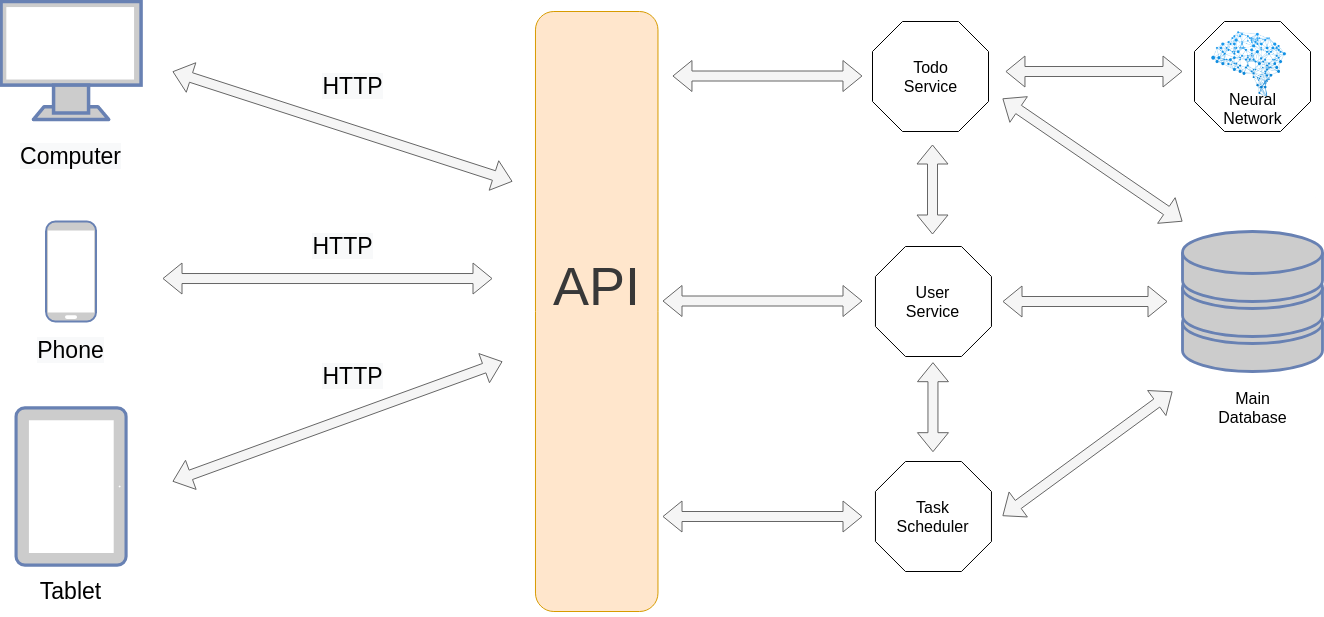
\includegraphics{Figures/abstract-architecture}}\\
		A High Level View of the Architectural organization
	\end{frame}
	
	%%%
	% Architecture  
	%%% 
	\begin{frame}{Architecture - Components }
		
		\vspace*{-4em} 
		
		\begin{itemize}
			\item \textcolor{sthlmBlue}{Client application:}
			\begin{itemize}
				\item Written in Typescript
				\item Angular 12 for the user interface
			\end{itemize}
			\item \textcolor{sthlmBlue}{Server application:}  
			\begin{itemize}
				\item Written in Typescript transpiled to Javascript for Node.js
				\item Neural Network written in Python
				\item Exposes a REST Web API to be used by the clients
				\item Uses PostgresSQL for the database
			\end{itemize}
			
		\end{itemize}
		
	\end{frame}
	
	%%%
	% Webapi
	%%% 
	\begin{frame}{Web API}
		
		\vspace*{-3em}
		\centering
		\scalebox{0.2}{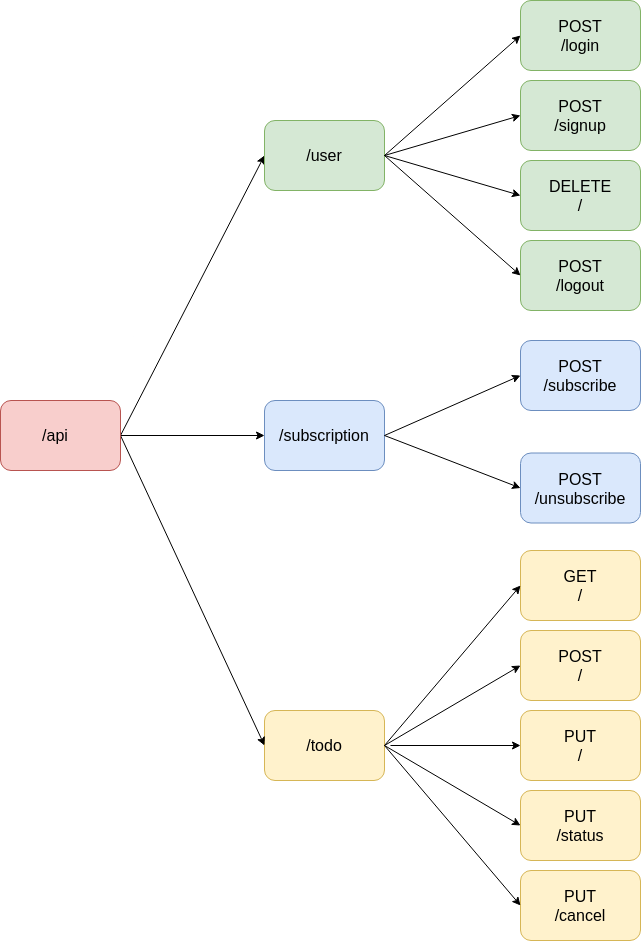
\includegraphics{Figures/web-api-abstract}}\\
		Overview of the API paths
		
	\end{frame}
	
	%%%
	% Conclusions
	%%% 
	\begin{frame}{Future Work}
		
		\vspace*{-5em}
		\begin{itemize}
			\item Mobile app
			\item Location synchronization
			\item Natural language comprehension
			\item Minor improvements
		\end{itemize}
		
	\end{frame}
	
	
\end{document}